\documentclass[11pt,a4paper]{article}
\usepackage{amsmath,amssymb,amsthm}
\usepackage{graphicx}
\usepackage[margin=2.2cm]{geometry}
\usepackage{xcolor}
\usepackage{titlesec}
\usepackage{fancyhdr}
\usepackage{booktabs}
\usepackage{enumitem}
\usepackage{float}
\usepackage{hyperref}
\hypersetup{colorlinks=true,linkcolor=blue!70!black,urlcolor=blue!70!black}

\renewcommand{\topfraction}{0.9}
\renewcommand{\bottomfraction}{0.9}
\renewcommand{\textfraction}{0.05}
\renewcommand{\floatpagefraction}{0.5}
\setcounter{topnumber}{3}
\setcounter{bottomnumber}{3}
\setcounter{totalnumber}{5}

\definecolor{primary}{RGB}{0,51,102}
\definecolor{accent}{RGB}{204,102,0}

\titleformat{\section}{\Large\bfseries\color{primary}}{\thesection}{1em}{}
\titleformat{\subsection}{\large\bfseries\color{primary!80!black}}{\thesubsection}{1em}{}

\pagestyle{fancy}
\fancyhf{}
\fancyhead[L]{\small\color{primary}Essential Summary}
\fancyhead[R]{\small\color{primary}Li \& Zhao (2011)}
\fancyfoot[C]{\thepage}
\renewcommand{\headrulewidth}{0.5pt}

\begin{document}
\raggedbottom

\begin{center}
{\LARGE\bfseries\color{primary}Essential Summary}\\[12pt]
{\large\bfseries Generalized Function Projective Synchronization\\of Two Different Hyperchaotic Systems\\with Unknown Parameters}\\[8pt]
{\normalsize Zhenbo Li, Xiaoshan Zhao}\\[4pt]
{\small\itshape Nonlinear Analysis: Real World Applications, Vol.\ 12, No.\ 5, 2607--2615 (2011)\\DOI: 10.1016/j.nonrwa.2011.03.009}\\[6pt]
{\small\rule{0.7\textwidth}{0.5pt}}\\[4pt]
{\small\color{accent}This is an author-prepared essential summary, not the original paper.\\Please cite the published version.}
\end{center}

\vspace{0.5em}

\section{Background and Motivation}

Projective synchronization is attractive for secure communications because its proportional feature enables fast communication. The concept evolved through several generalizations: \textbf{projective synchronization} (Mainieri \& Reh\'aczek, 1999, partially linear systems) $\to$ \textbf{modified projective synchronization} (MPS, constant scaling \emph{matrix}) $\to$ \textbf{function projective synchronization} (FPS, scaling \emph{function}) $\to$ \textbf{modified function projective synchronization} (MFPS, scaling function \emph{matrix}) $\to$ \textbf{generalized function projective synchronization} (GFPS).

This paper studies \textbf{GFPS between two different hyperchaotic systems whose parameters are completely unknown}. Combining adaptive control theory with an \textbf{antisymmetric structure}, the authors design an extended adaptive controller that is (i) more generalized than the controller in Yu \& Li (2010) and (ii) simpler than that in Du et al.\ (2009). Unknown parameters are simultaneously estimated.

\section{GFPS Scheme}

\subsection{Drive--Response Systems}

Drive system with unknown parameters $\Theta$:
\begin{equation}
\dot{x} = f(x) + \Phi(x)\Theta,
\label{eq:drive}
\end{equation}
Response system with unknown parameters $\Omega$ and controller $U$:
\begin{equation}
\dot{y} = g(y) + \Psi(y)\Omega + U.
\label{eq:response}
\end{equation}

\subsection{Error Definition}

The GFPS error is defined relative to a \textbf{scaling function matrix} $h(x) = \mathrm{diag}\{h_1(x), h_2(x), \ldots, h_n(x)\}$:
\begin{equation}
\boxed{e = y - h(x)x, \qquad \dot{e} = g(y) + \Psi(y)\Omega - J\big(f(x) + \Phi(x)\Theta\big) + U}
\label{eq:error}
\end{equation}
where $J = \mathrm{d}(h(x)x)/\mathrm{d}x$ is the Jacobian of the scaled state.

\textbf{Remark (hierarchy):} If all $h_i(x)$ are equal, GFPS $\to$ FPS. If all $h_i$ are constants, GFPS $\to$ MPS. If $h \equiv 0$, the problem reduces to chaos control. Thus GFPS unifies many existing schemes.

\section{Controller Design via Antisymmetric Structure}

\subsection{Stability Lemma}

\textbf{Theorem 1.} For $\dot{x} = B(x)x$ with $B(x) = B_1(x) + B_2$, if
\begin{itemize}[leftmargin=2em]
\item (i) $B_1^T(x) = -B_1(x)$ (antisymmetric),
\item (ii) $B_2 = \mathrm{diag}\{b_1,\ldots,b_n\}$ with $b_i < 0$,
\end{itemize}
and the invariant set contains only the origin, then the system is asymptotically stable.

\textbf{Proof.} With $V = \tfrac12 x^T x$, the antisymmetry of $B_1$ cancels the symmetric part:
\begin{equation}
\dot{V} = \tfrac12\big(x^T B^T x + x^T B x\big) = x^T B_2 x < 0.
\label{eq:lyap}
\end{equation}

\subsection{Main Controller (Theorem 2)}

GFPS is achieved by the controller and parameter update laws:
\begin{equation}
\boxed{U = J\big(f(x) + \Phi(x)\hat\Theta\big) - g(y) - \Psi(y)\hat\Omega + Ke}
\label{eq:controller}
\end{equation}
\begin{equation}
\dot{\hat\Theta} = -J^T \Phi^T(x) e + \tilde\Theta, \qquad
\dot{\hat\Omega} = \Psi^T(y) e + \tilde\Omega,
\label{eq:update}
\end{equation}
where $\hat\Theta, \hat\Omega$ are parameter estimates, $\tilde\Theta = \Theta - \hat\Theta$, $\tilde\Omega = \Omega - \hat\Omega$, and $K$ satisfies the assumptions of Theorem~1 (antisymmetric off-diagonal + negative diagonal).

\textbf{Proof.} Choose $V = \tfrac12(e^T e + \tilde\Theta^T\tilde\Theta + \tilde\Omega^T\tilde\Omega)$. Substituting the controller and update laws yields
\begin{equation}
\dot V = \tfrac12\big(e^T K^T e + e^T K e\big) - \tilde\Theta^T\tilde\Theta - \tilde\Omega^T\tilde\Omega < 0,
\label{eq:vdot}
\end{equation}
which guarantees global asymptotic stability of the error system and convergence of parameter estimates.

\textbf{Remarks.} The controller is simpler than Du et al.\ (2009) and more generalized than Yu \& Li (2010), whose controller is a special case. The scaling functions may be periodic or polynomial functions.

\section{Application: Hyperchaotic Chen $\to$ Hyperchaotic Lorenz}

The drive is a hyperchaotic Chen system and the response a hyperchaotic Lorenz system, both with fully unknown parameters:
\begin{equation}
\dot{x} =
\begin{pmatrix}
-a x_1 + a x_2 + x_4\\
d x_1 + c x_2 - x_1 x_3\\
-b x_3 + x_1 x_2\\
r x_4 + x_2 x_3
\end{pmatrix},
\qquad
\dot{y} =
\begin{pmatrix}
-a_1 y_1 + a_1 y_2 + y_4\\
b_1 y_1 - y_2 - y_1 y_3\\
-c_1 y_3 + y_1 y_2\\
d_1 y_4 - y_1 y_3
\end{pmatrix}
+ U.
\label{eq:systems}
\end{equation}
True parameter values: $a=35,\ b=3,\ c=12,\ d=7,\ r=0.08$; $\ a_1=10,\ b_1=28,\ c_1=\tfrac83,\ d_1=1.3$.

\subsection{Case 1: Periodic Scaling Functions}

\begin{equation}
h_i(x_i) = d_{i1}\sin(d_{i2}x_i + d_{i3}) + d_{i4}, \qquad i=1,2,3,4.
\label{eq:periodic}
\end{equation}

Figures~\ref{fig:fig1}--\ref{fig:fig3} show that the eight unknown parameters adapt to their true values and the synchronization errors converge to zero.

\begin{figure}[htbp]
\centering
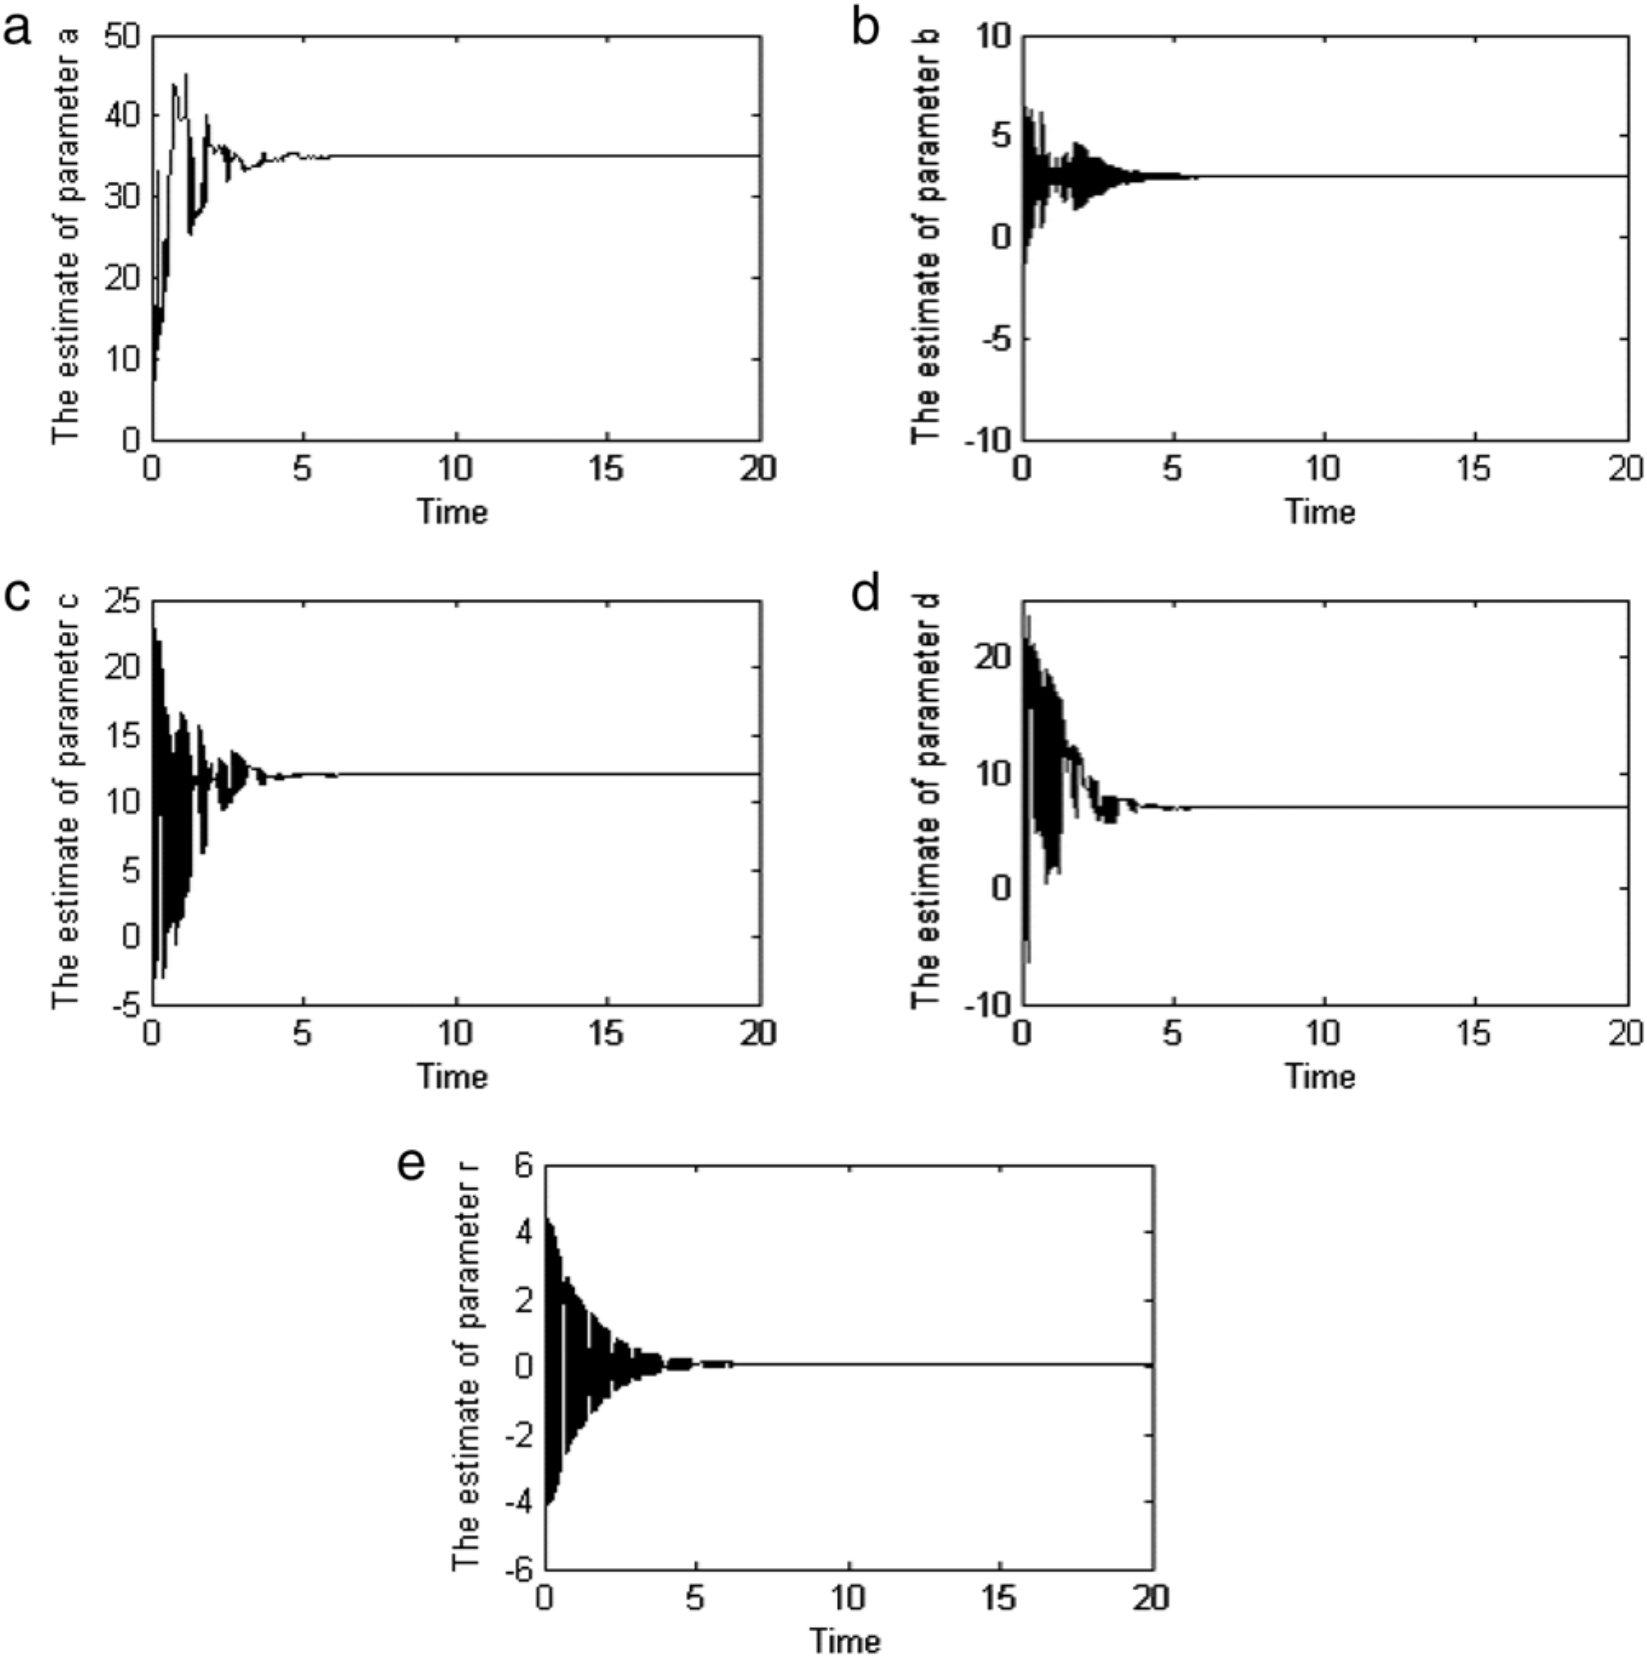
\includegraphics[width=0.85\textwidth,height=0.42\textheight,keepaspectratio]{nonrwa-fig1.png}
\caption{Estimation of the unknown parameters of the drive system (hyperchaotic Chen) under the parameter update law and periodic scaling functions.}
\label{fig:fig1}
\end{figure}

\begin{figure}[htbp]
\centering
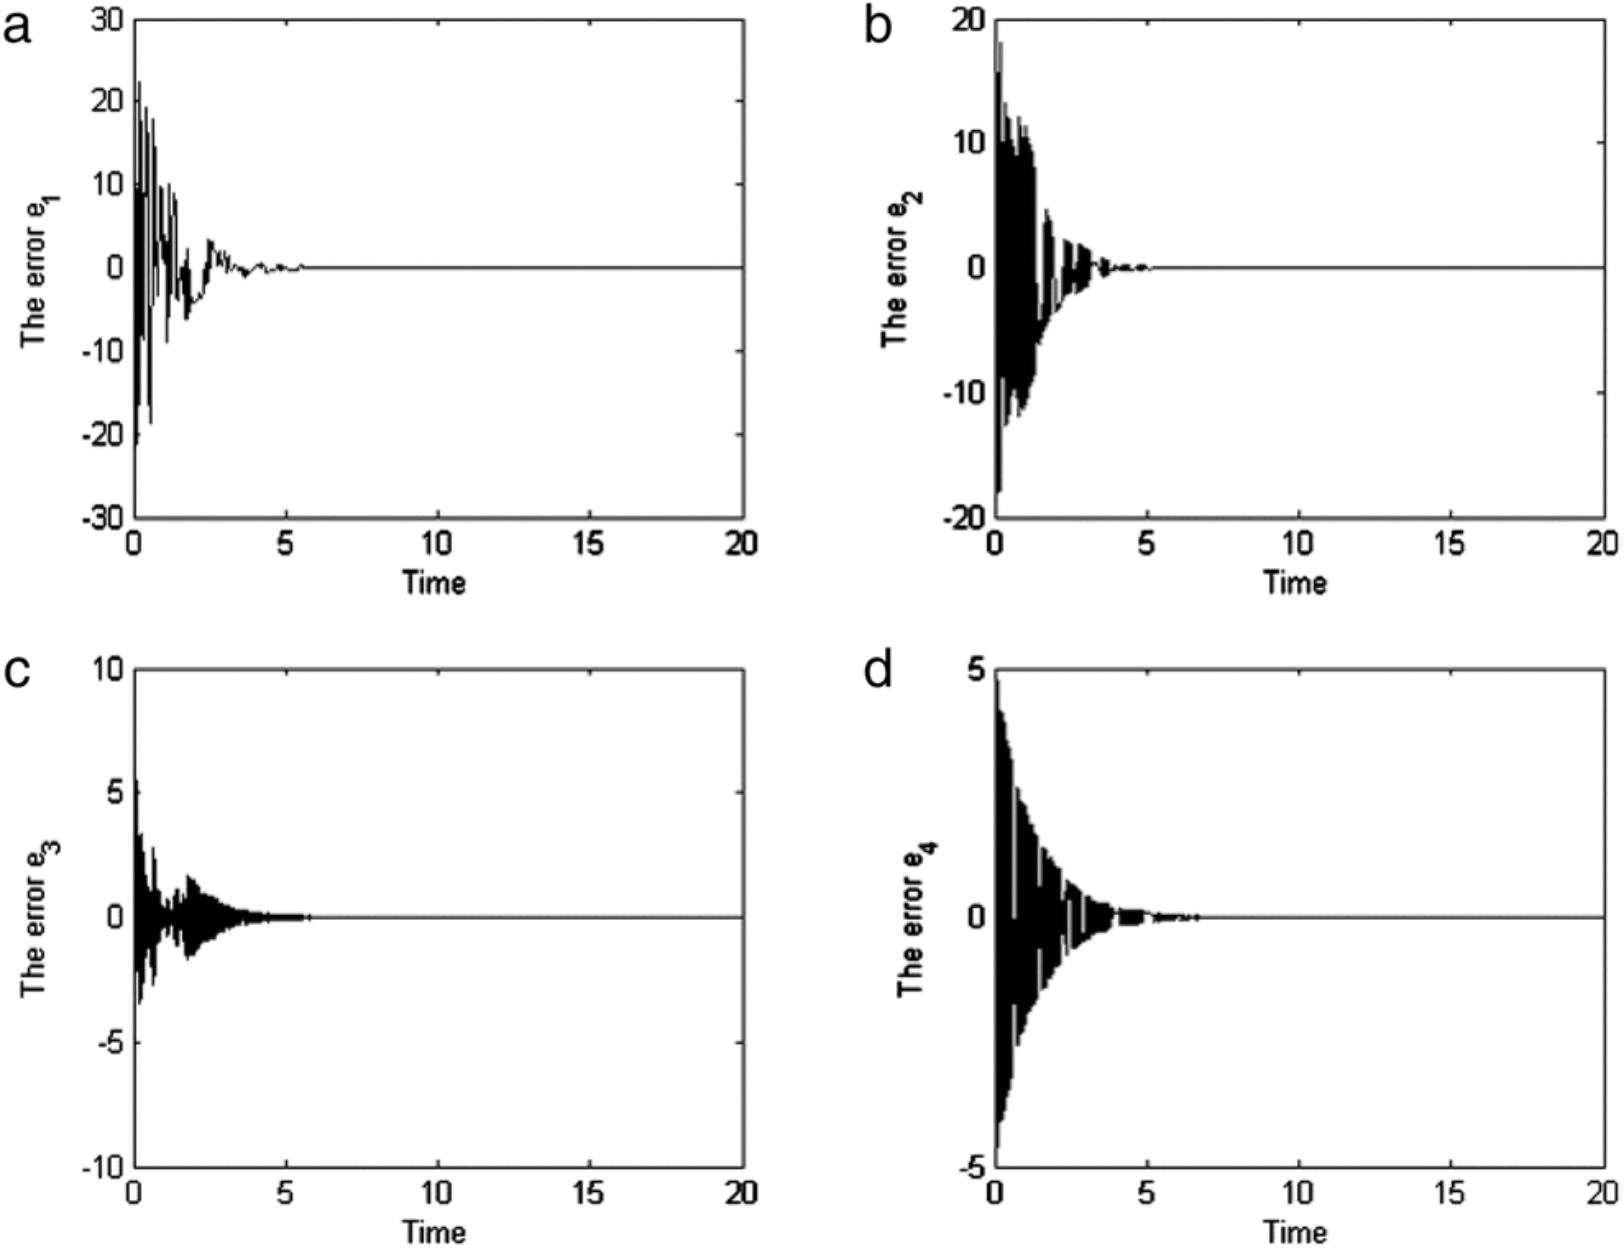
\includegraphics[width=0.85\textwidth,height=0.42\textheight,keepaspectratio]{nonrwa-fig3.png}
\caption{Time response of the generalized function projective synchronization errors between the two hyperchaotic systems with periodic scaling functions. The errors converge to zero as $t\to\infty$.}
\label{fig:fig3}
\end{figure}

\subsection{Case 2: Polynomial Scaling Functions}

\begin{equation}
h_i(x) = d_{i1}x_i^2 + d_{i2}x_i + d_{i3}, \qquad i=1,2,3,4.
\label{eq:poly}
\end{equation}

The corresponding parameter-estimation and error-response results confirm that GFPS is achieved and the unknown parameters are identified equally well.

\begin{figure}[htbp]
\centering
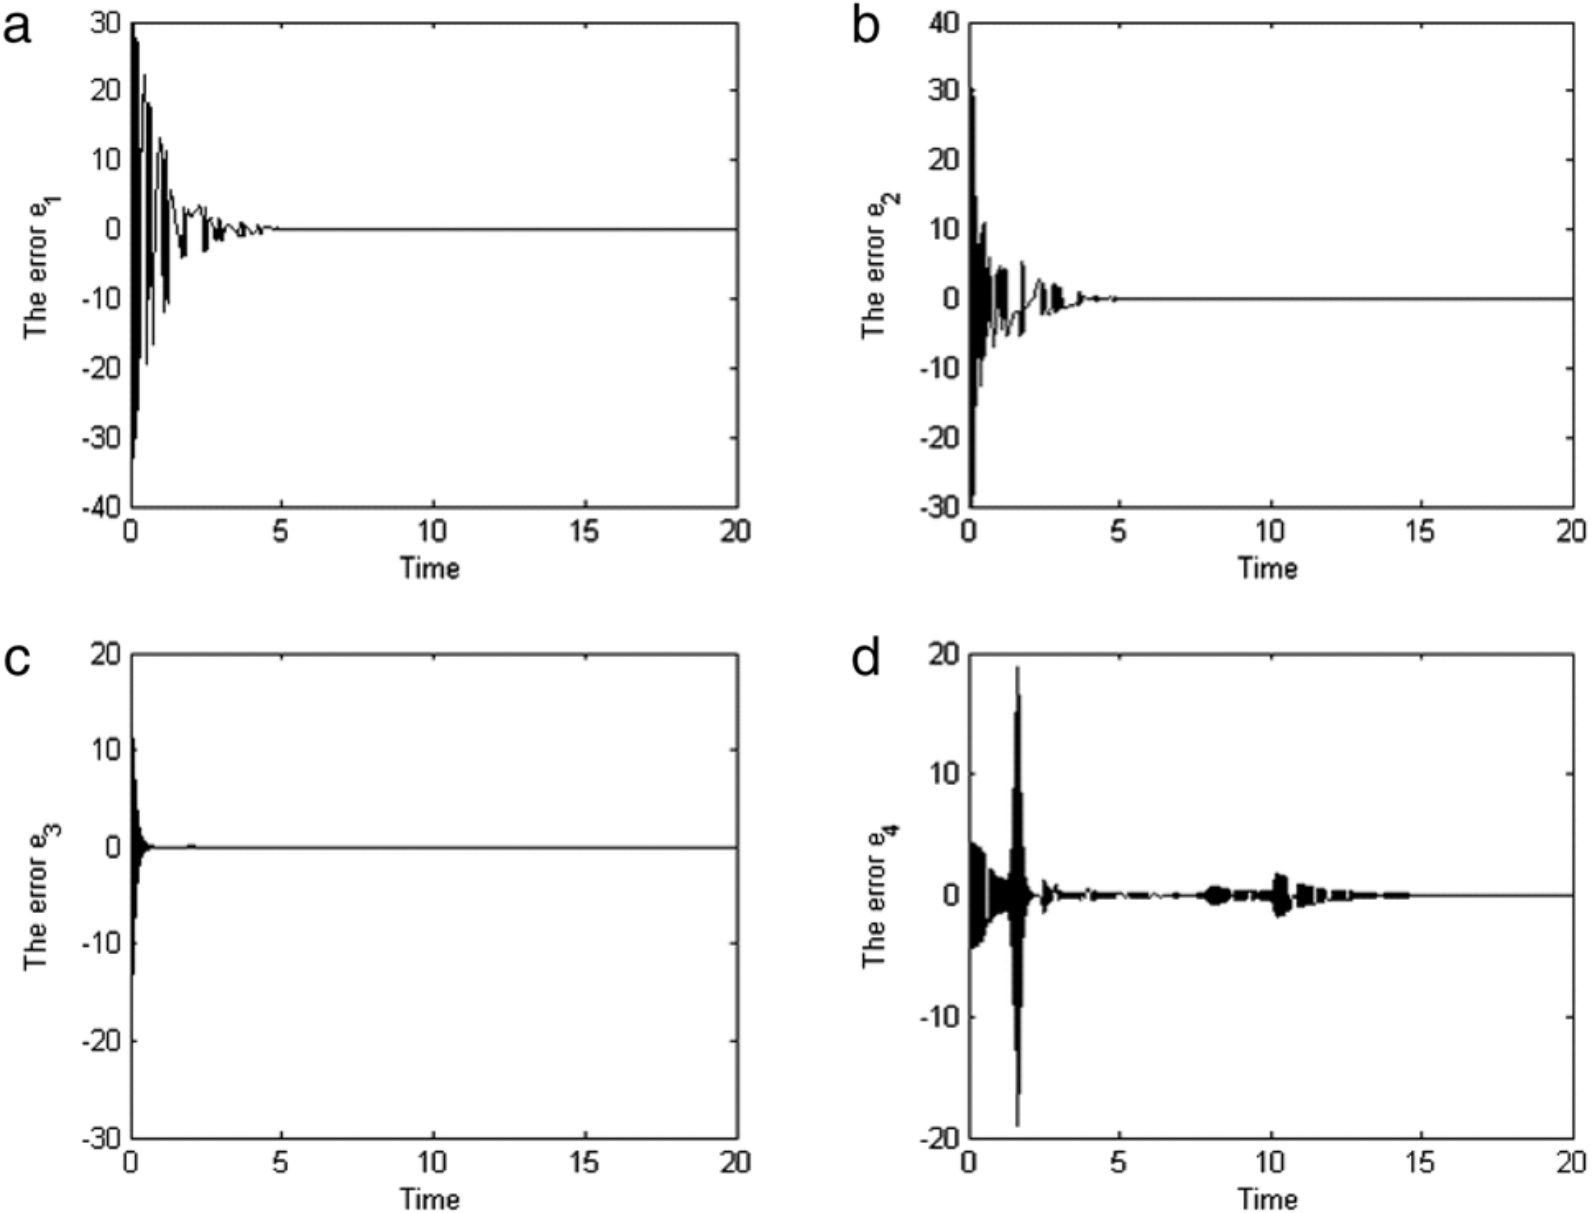
\includegraphics[width=0.85\textwidth,height=0.42\textheight,keepaspectratio]{nonrwa-fig6.png}
\caption{Time response of the generalized function projective synchronization errors with polynomial scaling functions.}
\label{fig:fig6}
\end{figure}

\section{Key Findings}

\begin{enumerate}[leftmargin=2em]
\item \textbf{Unified GFPS framework:} The scaling function matrix $h(x)$ generalizes FPS (scalar function), MPS (constant matrix), and chaos control ($h\equiv 0$) as special cases.

\item \textbf{Simpler, more general controller:} Combining adaptive control with the antisymmetric structure eliminates the need for complex matrix design. The controller is simpler than Du et al.\ (2009) and more general than Yu \& Li (2010).

\item \textbf{Parameter estimation for hyperchaotic systems:} All eight unknown parameters of the Chen and Lorenz hyperchaotic systems are simultaneously estimated while synchronization is achieved --- handled naturally by the adaptive update laws.

\item \textbf{Complicated scaling functions:} Periodic (sine) and polynomial scaling functions, which had not been discussed in prior literature, are both demonstrated to work.

\item \textbf{Lyapunov-based guarantee:} The antisymmetric structure ensures $\dot V = e^T B_2 e < 0$ (see Eqs.~\eqref{eq:lyap} and \eqref{eq:vdot}), giving a rigorous global asymptotic stability proof.
\end{enumerate}

\section{Significance}

This paper is the author's second major work in chaos synchronization (after the 2011 Acta Physica Sinica paper on modified active control for generalized projective synchronization). Together, these two papers establish the "chaos synchronization" thread in the author's research trajectory. The key methodological idea --- constructing controllers via an antisymmetric structure validated by Lyapunov theory rather than by algebraic eigenvalue criteria --- mirrors the same Lyapunov-centric design philosophy later applied to analytical perturbation methods (GHFP/MGHFP series).

\vfill
\begin{center}
\small\rule{0.5\textwidth}{0.3pt}\\[4pt]
\small\color{primary} Author: Zhenbo Li (lizhenbo@usc.edu.cn)\\
\small ORCID: 0000-0003-2290-971X\\
\small University of South China, School of Mathematics and Physics\\
\small Hunan Key Laboratory of Mathematical Modeling and Scientific Computing
\end{center}

\end{document}
